%!TEX root = ../main.tex

\chapter{The \gerda\ experiment}\label{chap:gerda}

The GERmanium Detector Array (\gerda) experiment has been proposed in
2004~\cite{gerda-proposal} to search for neutrinoless double-beta decay with High-Purity
Germanium detectors (HPGe) enriched in the \gesix\ double-beta emitter. The proposal lies
in the path opened by the Heidelberg-Moscow (\hdm)~\cite{Klapdor2001} and
\igex~\cite{Aalseth2002} experiments, aiming to develop the germanium technology towards
large-scale, \bkgfree\ experimental conditions that could tackle the scale of
$\mathcal{O}(10^{26})$~yr sensitivity on the neutrinoless double-beta decay half-life. The
history of the achievements in \thalfzero\ limit setting and background level with \gesix\
is presented in \cref{img:exp:ge76-history}, top. On the bottom plot, a zoom in the
\gerda\ data taking period showing the experimental progresses in terms of \thalfzero\
sensitivity, lower limit and collected active exposure.  \gerda\ data taking officially
ended in December 2019 after hitting the target total \bkgfree\ exposure of 100~\kgyr\ and
establishing itself as the leading experiment in the field in terms of lowest background
level ever achieved around \qbb~\cite{Agostini2019a}.

\blocktitle{\gerda\ \\ phases}
Since the start of the data taking in 2008 the experiment, located in hall~A of the Gran
Sasso National Laboratories (LNGS) in Italy, has been running through two distinct
experimental phases (\phaseone\ and \phasetwo). Detectors from the former \hdm\ and \igex\
experiments (of semi-coaxial geometry) along with newly produced diodes (of \bege\
geometry type, shorthand for Broad Energy Germanium detectors) were deployed bare into
liquid argon (LAr) during \phaseone, following a suggestion by ref.~\cite{Heusser1995},
for a total amount of 21.3~kg of germanium. \phaseone\ ended in June 2013 with a total
exposure of 21.6~\kgyr\ and a background index in the region of interest of
\pIbi~\cite{Agostini2016}.  Short after the upgrade works for \gerda\ \phasetwo\ started:
a new event veto system based on the LAr scintillation light was installed along with an
additional 20~kg of \bege-type detectors.  The newly designed veto system allowed for a
significant reduction of the background index (BI) down to the \powctsper{-4} scale, allowing
\gerda\ to seamlessly run in \bkgfree\ conditions for its full second experimental phase
and surpass the \powtenyr{26} sensitivity threshold in April 2018~\cite{Agostini2019a}.
Data taking was then stopped again to permit a third hardware upgrade, during which
another 9.6~kg of enriched germanium in the form of five inverted-coaxial geometry
detectors was deployed\footnote{Note however that a semi-coaxial detector (\ANG{1}) and
the natural \GTF{} detectors were removed.}. Moreover, the LAr veto system was exchanged
with a more efficient one, thanks to the denser fiber curtain and the addition of a shroud
enclosing the central string, now constituted by inverted-coaxial detectors. This last
part of \phasetwo, which will be referred as \phasetwop\ in the following, ended in
December 2019 after collecting the total exposure of \fillme{fillme}~\kgyr\ and
establishing the final \gerda\ upper limit on the neutrinoless double-beta decay half-life
of \gerdafinallimit. With that said, the ``\phasetwo'' period includes \phasetwop\ in the
following.
\begin{figure}
  \centering
  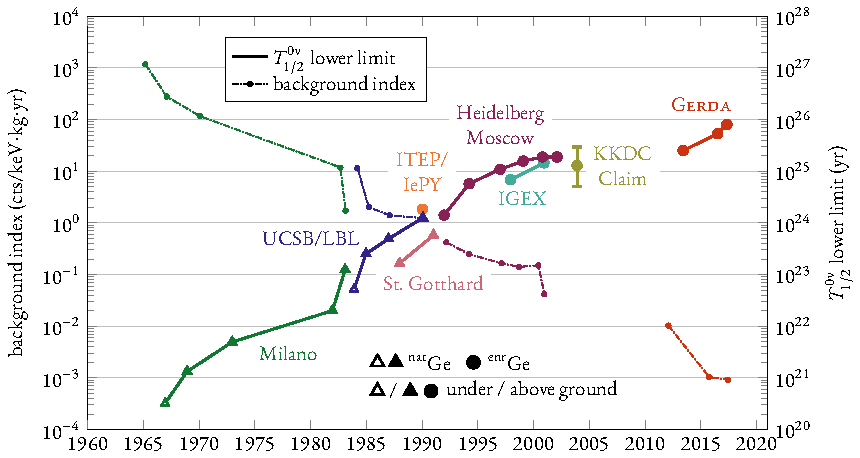
\includegraphics{plots/0nbb-ge76-history.pdf}
  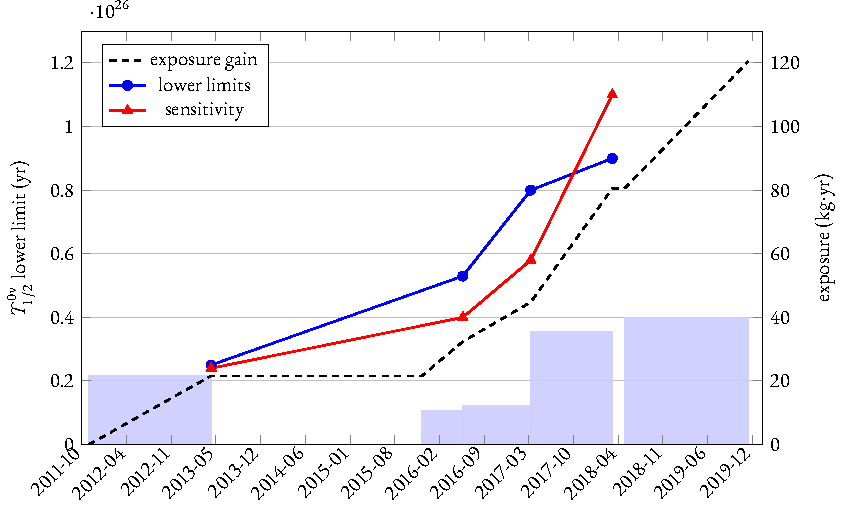
\includegraphics{plots/gerda-history.pdf}
  \caption{%
    Top: history of lower limits (68\% CL, 90\% CL since 1991) and background indices from
    \gesix\ neutrinoless double-beta decay experiments, extracted from~\cite{Fiorini1967,
    Bellotti1984, Caldwell1989, Reusser1991, Vasenko1989, Klapdor2001, Aalseth2002,
    Klapdor2004, Alvis2019, gerda-final} and references therein. Original design by Karl-Tasso
    Kn\"opfle.  Numbers attached to single data points correspond to exposures in
    mol(\gesix)$\cdot$yr. Bottom: evolution and milestones set by the \gerda\ experiment
    through its three experimental phases. The exposure gain, the neutrinoless double-beta
    decay half-life sensitivities and upper limits are tracked over time. \fillme{to be
    updated}
  }\label{img:exp:ge76-history}
\end{figure}
\newpar
The \phasetwop\ upgrade is partly also a test bench for the next-generation successor of
\gerda\ in the field of double-beta decay physics with \gesix, the LEGEND experiment. The
collaboration, formed in October 2016 from the \gerda\ and \majorana~\cite{Abgrall2014}
(the latter experiment searching for \onbb\ with germanium detectors at the Sanford
Underground Research Facility (SURF) in USA), pursues the goal of building a tonne-scale
\gesix\ experiment and reaching the $\mathcal{O}(10^{28})$~yr sensitivity scale. The first
phase of the experiment, LEGEND-200, deploys 200~kg of germanium in the existing \gerda\
infrastructure at LNGS and it is currently in commissioning phase.
\newpar
As the present thesis work focuses on \gerda\ \phasetwo\ data, the description of the
experimental setup and the main analysis techniques given in the following will be limited
to that time period. The chapter is structured as follows. In \cref{sec:gerda:setup} a
general overview of the \gerda\ \phasetwo\ (and \phasetwop) apparatus is given. In
\cref{sec:gerda:cuts} the working principles of the main background reduction techniques
that allow \gerda\ to operate in the background-free regime are outlined. The application
of these event-selection criteria to the \phasetwo\ data is then described in
\cref{sec:gerda:ana}, and the final results are presented.

\section{Overview of the Phase {\normalfont\textit{II}} experimental setup}%
\label{sec:gerda:setup}

The \gerda\ experiment is located in hall~A of the LNGS laboratories, at a depth of about
3500~m water equivalent, to suppress cosmogenically-induced background
sources~\cite{Wiesinger2018}. The germanium detectors are arranged into strings within a
cryostat filled with 64~m$^3$ of liquid argon (LAr), which acts as a shielding and cooling
medium at the same time. The cryostat itself is enclosed by a large tank containing
590~m$^3$ of ultra-pure water.  Besides the additional shielding effect, this water layer
act as a medium for a \v{C}erenkov veto system with 66 photomultiplier tubes (PMTs)
against muons. An array of scintillating panels is installed on the top of the clean room
to complete the muon veto system~\cite{Freund2016}. A simplified representation of the
experimental setup is given in \cref{fig:setup:overview}, together with a picture taken
from the outside.

\begin{figure}
  \centering
  \includegraphics[width=\textwidth]{setup/gerda-overview.pdf}
  \caption{%
    On the right: artist view of the \gerda\ experimental setup. On the left: a picture of
    taken during the inauguration in November 2010. The experiment, installed in hall A of
    the Gran Sasso National Laboratories in Italy, deploys an array of germanium detectors
    enriched in \gesix\ bare in liquid argon, together with a liquid argon scintillation
    light veto system. The cryostat is submerged in a water tank to provide additional
    shielding from external background sources. A plastic scintillating panel system is
    installed on the top of the whole structure as an active muon veto, together with the
    water tank.
  }\label{fig:setup:overview}
\end{figure}

\blocktitle{detectors}
The \gerda\ \phasetwo\ array is organized in 7 vertical strings, holding 40 detectors in
total. The detectors can be divided in three groups: the \bege\ detectors, the
semi-coaxial \m{ANG} and \m{RG}, and the semi-coaxial \m{GTF} detectors. The
detectors of the first two groups are made of germanium enriched in \gesix, the third
group includes detectors with natural isotopic germanium abundance.
\newpar
All \gerda\ HPGe detectors are made of high-purity p-type germanium, which is initially
used to pull crystals, typically fuse-shaped (see for example fig.~4.1a in
\cite{Yonenaga2019}).  Crystals are then cut in slices, and each of them is further
processed to obtain the final detector geometry. The electrodes for signal read-out and
voltage biasing are then fabricated on the detector surface. The \nplus\ contact, where the
external voltage is applied, `wraps around' the detector. It is obtained by deposition of
a lithium layer on the surface, which diffuses below the surface until a depth of
$\sim$1~mm during the subsequent thermal annealing cycles. The presence of lithium
impurities effectively creates a region with decreased charge collection efficiency (CCE),
or `dead-layer', even when biased at full-depletion voltages.  In this region, the CCE is
zero at the surface and reaches its maximal value at the full charge collection depth
(FCCD). The \pplus\ electrode, where the signal is read out, is instead fabricated by boron
implantation, and the dead layer it produces is typically smaller, at the level of
hundreds of microns. The two conductive surfaces are separated by an insulating region,
which is typically produced by excavating a `groove'. In some cases such groove is
passivated by deposition of a germanium-oxide layer.

\blocktitle{%
  \includegraphics[width=13mm]{gedet/BEGe.png}\\
  \includegraphics[width=13mm]{gedet/SemiCoax.png}%
}
The \gerda\ \phasetwo\ detectors can be classified according to two different geometry
types: semi-coaxial and \bege. In the semi-coaxial design, a bore-hole is excavated along
the central axis to accomodate the \pplus\ electrode. With such a configuration,
relatively large detector masses can be achieved, of the order of 2--3~kg. The \ANG{} (5),
\RG{} (2) and \GTF{} (3) detectors, inherited from the \hdm\ and \igex\ experiments and
already used in \phaseone, are of the semi-coaxial type. Their total mass amounts to
23.2~kg of germanium, while the enrichment fractions are in the 85.5--88.3\% range. For
\phasetwo, 20~kg of germanium enriched at 87.8\% was procured by the \gerda\ collaboration
for the production of 30 new diodes of the \bege\ type. The Broad Energy Germanium detector
design does not include a bore-hole, therefore the \pplus\ contact is a small, dot-shaped
surface at the center of one of the two detector sides. The absence of a bore-hole makes
this kind of detectors harder to fully deplete, requiring lower impurity concentrations
and smaller masses, generally lower than 1~kg. A detailed description of the
characteristics of the \bege\ detectors, from germanium procurement to diode production can
be found in~\cite{Agostini2015e, Agostini2018a, Agostini2019}.

\begin{figure}
  \centering
  \includegraphics[height=7cm]{gedet/phII-array.png}
  \hspace{0.5cm}
  \includegraphics[height=6cm]{gedet/phII-array-2D.pdf}
  \caption{%
    The \gerda\ \phasetwo\ detector array.
  }\label{fig:setup:array}
\end{figure}

\blocktitle{array \\ instrumentation}
As already mentioned, the \gerda\ \phasetwo\ detectors are arranged into 7 strings, packed
closely together as depicted in \cref{fig:setup:magevolumes}a, to maximize the
multi-detector event rejection efficiency. Since the main background sources in
\phaseone\ were located close to the detectors, the design of the mounting and cabling
system has been carefully chosen to minimize the mass. The detector holder unit consists
of a low-mass, intrinsically radio-pure silicon plate and three vertical copper bars to
take the detector weight and connect the modules between themselves within a string. The
silicon plate provides the substrate onto which signal and high voltage cables are
attached. The Ge detectors are read out with custom-produced, cryogenic and low
radioactivity preamplifiers called `CC3'~\cite{Riboldi2015}. The Ge readout electrode is
connected to the JFET-PCB by a flexible flat cable. Two different cable types are adopted
for the signal and HV contact: the HV cables are made from 10 mils Cuflon\reg, or 3 mils
Pyralux\reg, the signal FFCs from 3 mils Cuflon\reg\ or Pyralux\reg. See
\cref{fig:setup:magevolumes}b.

\blocktitle{LAr veto}
To improve the sensitivity on the \onbb\ half-life and operate in the \bkgfree\ regime, an
additional active veto system to collect the LAr scintillation light produced by
background events was designed and installed during the upgrade works for \phasetwo. A
cylindrical hybrid design was chosen to detect the light information: a curtain made of
light-guiding plastic fibers coupled to a ring of silicon photomultipliers (SiPMs) to
surround the array and PMTs on the top (9) and on the bottom (7) (see
\cref{fig:setup:magevolumes}f). To enhance the light collection efficiency two copper
shrouds (visible in \cref{fig:setup:magevolumes}e) coated with a reflective Tetratex\reg\
layer were added between the fiber shroud and the PMT holder plates. The latter were
coated with a reflective VM2000 layer. Another light collection improvement introduced by
the \phasetwo\ upgrade is the installation of nylon (mini-)shrouds enclosing each detector
string (\cref{fig:setup:magevolumes}d). The presence of these shrouds provides an
essential mechanical barrier to reduce the background from \kvz\ ions naturally present in
LAr, which undergo \b-decay and can mimic the \onbb\ signature at \qbb. Being made of
transparent nylon material, in contrast to the ones from \phaseone\ made of copper, the
mini-shrouds let the light propagate more efficiently to a close-by light collecting
surface. To match the fibers and PMTs spectral response many surfaces in the close vicinity
of the array were coated with tetraphenil-butadiene (TPB), a wavelength shifting material.
Coating has been applied on mini-shrouds, fiber-shroud, copper shroud, PMTs as well as
their holder plates. The reader is referred to ref.~\cite{Agostini2018a} for the detailed
LAr veto instrumentation technical specifications.

\begin{figure}
  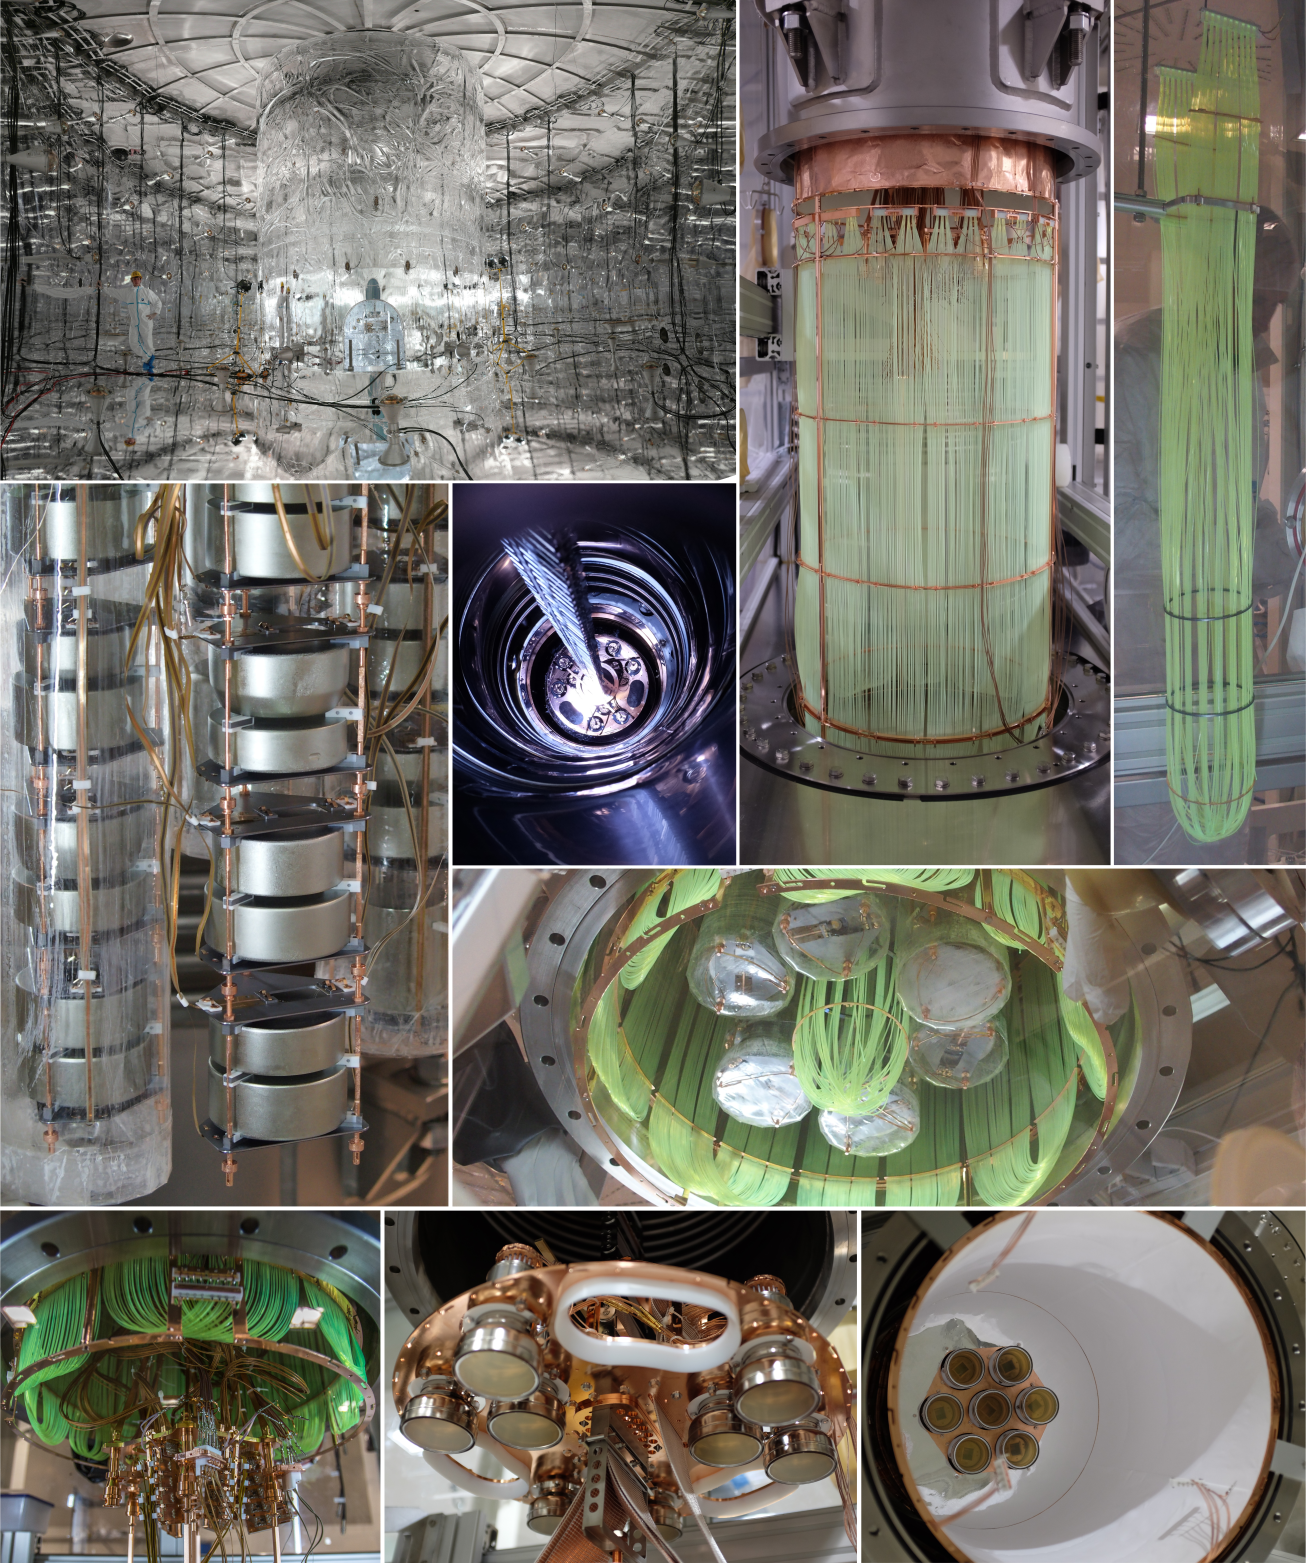
\includegraphics{setup/pic-collage.pdf}
  \caption{%
    Various pictures of the \gerda\ \phasetwo\ setup, taken during the upgrade
    works.
  }\label{fig:setup:pictures}
\end{figure}

\blocktitle{calibration \\ system}
The \gerda\ weekly calibrations are performed by lowering three \Th\ sources into LAr in
the close vicinity of the array, at the same radial distance from the array central axis
and evenly spaced. Each source, when lowered, just fits into the space between the
cylinder of the LAr veto system and two neighboring outer strings of the detector array,
thereby the sources enter the inner volume of the LAr veto system by three slots in the
top PMT plate.  The three sources were produced for \phasetwo\ and
characterized~\cite{Baudis2015}. The LAr veto instrumentation is usually switched off
during calibration runs because of the too high source activity of $\mathcal{O}(10)$~kBq.
However, less intense \Ra\ sources are also available and can be easily exchanged with the
standard ones. Special calibration data has been acquired with these sources and the LAr
light instrumentation turned on, to study the performance of the LAr veto system. The
calibration of the experimental setup is extensively described in ref.~\fillme{[fillme]}.

\blocktitle{data \\ acquisition}
A FADC system records traces from germanium detectors (40), PMTs (16) and SiPMs (15) of
the LAr veto, PMTs and scintillating panels of the muon veto when an energy deposition
greater than about 100~keV occurs in at least one of the germanium detectors\footnote{The
exact trigger threshold is detector- and run-dependent and varies between 20~keV and
200~keV.}.  The energy deposition associated to each germanium detector signal is
determined via a Zero Area Cusp (ZAC) filter which is optimized off-line for each detector
and each calibration run~\cite{Agostini2015}. PMT and SiPM hits are reconstructed in the
offline analysis following the procedure documented in~\cite{Agostini2018a}. Each event
has to pass a series of quality cuts tailored to discard unphysical events such as
discharges, pile-up, overflowed events and other problematic traces with very high
efficiency (estimated to $(99.902 \pm 0.002)$\% \fillme{how?}). The
reconstructed trigger positions are converted into time differences relative to the first
trigger found in the germanium detector traces. Trigger positions and amplitudes are
subsequently used together with hits from the SiPM to test the LAr veto condition. The
algorithms were implemented in the \gelatio\ framework~\cite{Agostini2011} which is used
to process \gerda\ data. Each event is characterized by the calibrated energy deposited in
the Ge diode, a data quality flag, the classification as signal or background event from
the pulse shape analysis, and veto flags from the muon veto and LAr veto systems.

\begin{figure}
  \centering
  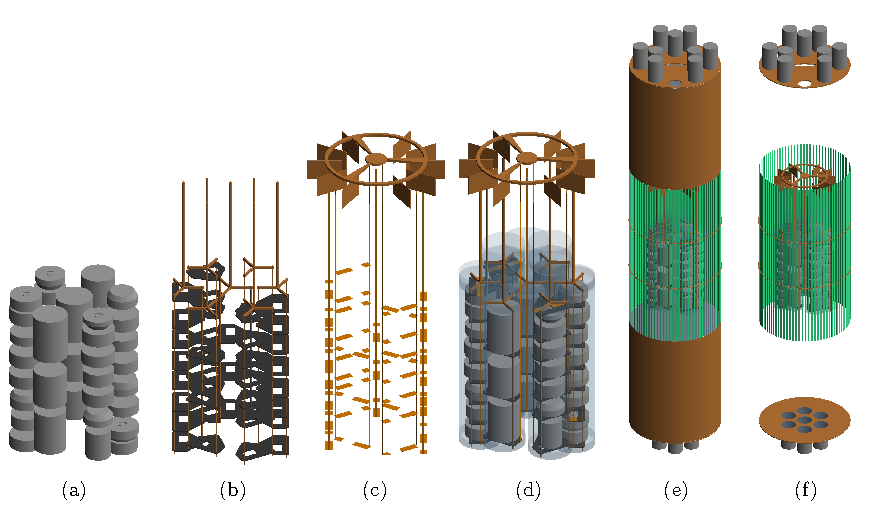
\includegraphics[width=\textwidth]{setup/mage-volumes.pdf}
  \caption{%
    Implementation of the \gerda\ array in \mage, visualized using the
    \geant\ visualization drivers. From left to right: a) the \gerda\
    detectors, b) the holder mounting, composed of silicon plates and
    copper bars c) the high-voltage and signal flexible flat cables plus
    the front-end electronics on top, d) the full array instrumentation,
    including the transparent nylon mini-shrouds, e) the full LAr veto
    system surrounding the array, including the fiber shroud (in green),
    the Tetratex\reg-coated copper shrouds (above and below the fibers) and
    the two PMT arrays, f) the LAr veto system without the copper
    shrouds.%
  }\label{fig:setup:magevolumes}
\end{figure}

\section{Background reduction techniques}%
\label{sec:gerda:cuts}

\begin{figure}
  \centering
  \includegraphics[width=\textwidth]{gedet/gerda-events.png}
  \caption{%
    Signal and background events in \gerda, working principles of the main background
    reduction techniques. From left to right: \emph{signal-like events}: the point-like
    topology in dense detectors of double-beta decays generate distinct single-detector
    pulse shapes. \emph{granularity cut}: external, background \g{}s can deposit energy
    in multiple detectors. \emph{pulse-shape discrimination}: insights on the event
    topology can be obtained by analyzing its waveform. Single-site events, multi-site
    events, \b{}s and \a{}s on the surface can be discriminated with offline algorithms
    depending on the specific detector geometry. \emph{LAr veto}: background events that
    deposit energy in germanium and LAr at the same time can be efficiently vetoed by
    the \gerda\ LAr veto.
  }\label{fig:gerda:event-types}
\end{figure}

Various background mitigation techniques are adopted, both at the data acquisition level
(online) and the analysis level (offline) in \gerda\ to lower the background index to the
`background-free' level of \pIIbi.

\blocktitle{muon veto}
Muons may cause a substantial background to rare event searches like \gerda\ by generating
counts at \qbb\ either through direct energy deposition in the detectors or through
e.g.~decay radiation of spallation products. At LNGS the cosmic muon flux is reduced by a
factor of ${\sim}10^6$ to a rate of ${\sim}3.4 \cdot 10^{−4}~\text{s}^{-1}\text{m}^{-2}$,
which is sill sufficient to generate a non-negligible background of the order of
\powctsper{-3}.  As already described in \cref{sec:gerda:setup}, a muon veto comprising of
a water \v{C}erenkov veto and a scintillator veto was implemented in \gerda\ to reduce
this background contribution. An event with energy deposition in germanium is flagged
as muon-induced background if a coincidence with the muon veto signal occurs in a $\pm
10$~\mus\ window around the germanium trigger. The efficiency of the muon veto system
has been estimated to be of ${\sim}99$\%, leading to a residual background index of
${\sim}$\powctsper{-5}~\cite{Freund2016}.

\blocktitle{LAr veto}
The primary role of liquid argon in \gerda\ is to keep the germanium detectors at a
cryogenic operational temperature and provide a passive shielding medium against external
backgrounds. Moreover, the LAr can be also employed as a detector medium in an active veto
system, thanks to its scintillation properties. The production mechanism of the
scintillation light in LAr is known since several decades and is deeply described in
literature and its spectrum is today well known. The incident particles deposit their
energy mainly by interactions with the electron shell of the argon atoms which leads to
either an excitation or an ionization of argon atoms. Excited argon atoms are frequently
called `excited dimers' or `excimers' in the literature. Their decay is accompanied by the
emission of scintillation light in the vacuum ultraviolet region, whose typical wavelength
is usually cited as $\lambda = 128$~nm~\cite{Heindl2010}. The ratio between excitation and
ionization is strongly dependent on the pressure and density of the argon as well as on
the type of radiation itself. In the case of excitation, the excited argon atom can
directly form an excimer via the collision with neighboring argon atoms. The process is
sketched in \cref{fig:setup:lar-scint}.
\begin{figure}[h]
  \centering
  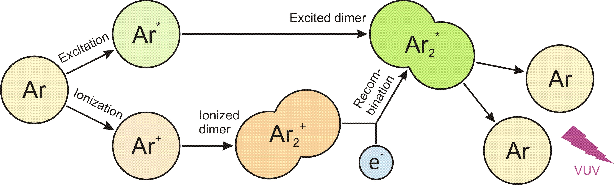
\includegraphics[width=0.7\linewidth]{lar-scint-mechanism.pdf}
  \caption{%
    Scintillation mechanism of liquid argon (or gaseous argon) via the decay of excited
    dimers. The excited dimer can be either formed directly from an excited argon atom or
    from an ionized atom which forms an ionized dimer before its recombination and the
    following recombination in its molecular form. Drawing courtesy of Christoph
    Wiesinger.
  }\label{fig:setup:lar-scint}
\end{figure}
The excimer itself is meta-stable and appears in two different states: the singlet and the
triplet state~\cite{Jortner1965, McCusker1984}.  The decay of the triplet state is
forbidden due to angular momentum conservation, while the decay of the singlet state is
allowed. Consequently the lifetime of the triplet state is 1.59~\mus\ which is
significantly higher than the 6~ns of the singlet state. The scintillation light yield
(combined for both components) is roughly 40 photons/keV, measured in ultra-pure
LAr~\cite{Doke1988}. This value is dependent on different factors, like the presence of
contaminants, the pressure and density of the argon as well as the ionization density of
the incident particle~\cite{Doke1988}.
\newpar
The goal of the \gerda\ LAr veto is to reject those types of background events in the
germanium detectors that simultaneously deposit energy in the surrounding LAr, and hence
generate scintillation. These background types mainly include \g-ray background from Ra
and Th decays in solid materials inside and around the detectors. But also other types of
background can successfully be rejected, such as muons or decays from \Arh\ or \kvz. An event
depositing energy in the germanium detectors is discarded as background if a coincidence
with the LAr veto signal is found in the time window spanned by the germanium traces.
Since the lifetime of the LAr triplet state significantly depends on the argon
purity~\cite{Amsler2007}, it is possible to monitor the purity of LAr over time.
\cref{fig:lar:triplet-lifetime} shows the lifetime values measured every month since
the start of \phasetwo. \fillme{comment}.
\begin{figure}
  \centering
  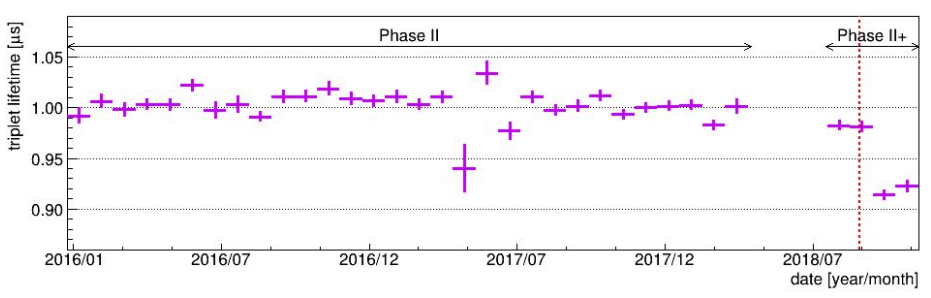
\includegraphics[width=0.8\linewidth]{plots/lar-triplet-lifetime.png}
  \caption{%
    \fillme{to be updated} LAr triplet lifetime regularly measured during \phasetwo.
  }\label{fig:lar:triplet-lifetime}
\end{figure}
The efficiency of the LAr veto cut can be estimated by evaluating the number of test
pulses that are randomly flagged as background events. For \phasetwo\ this fraction has
been evaluated to 97\%, corresponding to an efficiency for \onbb\ events of
\[
  \epsilon_\onbbM^\text{LAr-veto} = \fillme{fillme} \;.
\]

\blocktitle{pulse-shape \\ discrimination}
The drift of charges created by a ionizing particle in a voltage-biased germanium
detector, which determines the shape of recorded event waveform, depends on the electric
field in the diode. The latter, in particular, depends on the geometry and on crystal
parameters like the impurity concentration and its gradient. Therefore, analysis
techniques can be developed to discriminate between various event types in germanium
detectors. Distinguishing between single-site (SSE) and multi-site (MSE) events is of
primary interest for \gerda, since \onbb\ decays pertain to the SSE class. The two
electrons, in fact, deposit their energy in germanium within 1~mm$^3$ and can be therefore
considered as point-like events. On the other hand, background events caused by
e.g.~multiple Compton scattering of external \g\ rays are mostly of the multi-site type.
Besides MSEs, surface events are another prominent source of background. Energetic \b\
rays created at the \nplus\ electrode surface can penetrate the dead-layer and deposit
energy in the active volume. In particular, the \b\ decay of \kvz, a daughter of \Arh\
naturally present in LAr, is a dangerous background in the ROI because of its high
Q-value. These \b\ decays at the \nplus\ surface can create `slow' pulses with incomplete
charge collection because of the low electric field in the Li-diffused region. The \pplus\
electrode and the insulating groove can be trespassed also by \a\ particles. The
shallowness of the boron implantation of the \pplus\ (hundreds of nanometers) and the
absence of any dead layer in the groove\footnote{The passivation layer, if present, is
usually hundreds of nanometers thick and can be therefore penetrated by \a\ particles.}
let external \b{}s and \a{}s deposit energy in the detector active volume. The intense
electric field causes energy depositions in this region to generate pulses with short
rise times. \a\ events on the \pplus\ electrode are mainly produced by \Po\ accumulated
on its surface, most probably during detector handling. These 5.3~MeV \a\ particles may
lose part of their energy before reaching the active volume and contribute to the
background in the ROI.
\newpar
To mitigate all these background sources, pulse-shape discrimination (PSD) techniques were
developed separately for \bege\ and \scoax\ detectors separately, to be applied after the
LAr veto cut. For the first class a simple univariate cut was sufficient, while for the
latter two techniques were worked out, one based on neural networks and one on the
analysis of the rise time of the pulses.  In order to avoid systematic effects
calibration, training and evaluation of the PSD methods should be performed on pulses with
energies close to these of the expected signal at \qbb.  In practice, appropriate event
sets are extracted from the weekly \Th\ calibration spectra. The PSD methods applied to
the \gerda\ data are briefly outlined in the following. The interested reader is referred
to~\cite{psd-paper} for a detailed treatment of the topic.

\blocktitle{PSD for \\ \bege{}s}
PSD for the \bege\ detectors is based on the \aoe\ ratio, where $A$ is the maximum
amplitude of the current signal and $E$ is the event energy. This technique has been
extensively studied in the past in the context of \gerda~\cite{Agostini2013, Agostini2010,
Budjas2008, Budjas2009, Budjas2009a, Agostini2010}. The motivation in employing such a
relatively simple, univariate cut lies in the observation that in the \bege\ detectors,
thanks to their small \pplus\ contact, the electric field has a special distribution,
resulting in the same shape of pulses induced by drifting holes along paths near the
\pplus\ electrode~\cite{Agostini2010}. Multiple energy depositions in the detector can be
treated as a superposition of several single interactions. It follows that a MSE will have
a lower $A$ compared to a SSE with the same $E$.  A two-sided cut on \aoe\ to cut MSEs
slow pulses and \pplus\ fast events is introduced and determined separately for each
detector. Energy and time stability corrections to \aoe\ are discussed in detail
in~\cite{psd-paper}. As mentioned before, the \aoe\ cut values are determined employing
representative data samples from \Th\ calibration runs.  The low cut position (rejection
of MSEs and slow pulses) is adjusted to achieve a 90\% survival fraction of the
double-escape peak (DEP), a SSE sample. The determination of threshold on the high \aoe\
side (rejection of fast pulses) depends on the specific \phasetwo\ dataset and is
documented in~\cite{psd-paper}. The survival fraction for the \onbb-decay signal has been
calculated assuming that it is the same as for the DEP events. A full analysis of the
statistical and systematic uncertainties yields:
\[
  \epsilon_\onbbM^{A/E} = (87.6 \pm \stat{0.1} \pm \syst{2.6}) \% \;.
\]

\blocktitle{PSD for \\ \scoax{}s}
In semi-coaxial detectors the length of the drift path of the holes depends on the
location of the energy deposition and it induces different types of pulse shapes. Because
of this reason, a simple \aoe\ cut would not be as effective as for the \bege{}s, and
therefore alternative methods have been worked out.
\newpar
The primary method to reject MSE, called here \annmse, is based on an TMVA-based
artificial neural network\footnote{\url{https://root.cern/tmva}} implemented and requires
appropriate selection of input variables (from the rising part of the preamplifier charge
pulse) and training on independent data samples. Several of these samples are available
for training in calibration data (see \fillme{fillme}) and also in physics data (\kvz\
full-energy peak, \nnbb\ events, \a-induced events). The \annmse\ is specifically trained
on \Th\ calibration data, selecting the \Tl\ DEP as a SSE sample and the \Bil\ FEP at
1621~keV as a MSE sample. The classifier cut threshold is then fixed to a 90\% survival
probability for the \Th\ DEP, and the cut signal efficiency is calculated from Monte Carlo
simulations of \onbb-decay events. The obtained \annmse\ signal survival fraction is $(85
\pm 5)$\%.
\newpar
\a-induced events on the \pplus\ electrode surface are rejected by a separate method based
on the analysis of the pulses rise time (RT). These events are generally characterized by
a fast collection time, and their charge collection might be delayed or partial, if
originated in the proximity of the groove. The RT cut exploits the fast rise time of these
\a\ events and is therefore equivalent to a volume cut, which excludes the surfaces
vulnerable to the \a-induced events. The rise time is defined as the time the waveform
needs to reach from 10\% to 90\% of its amplitude. The RT-cut threshold is defined to
maximize the \onbb\ survival fraction and to minimize the signal-to-noise ratio at the
same time through the definition of a figure of merit defined as the product of the \nnbb\
signal survival probability and the \a-events rejection probability. The \nnbb\ and
\a-event test samples are obtained from physics data by selecting data in the $[1.0,
1.3]$~MeV and $>3.5$~MeV energy regions, respectively, after \annmse\ and LAr veto cuts.
The \onbb-signal efficiency of the RT cut is assumed to be the same as for the \nnbb\
decays and hence estimated to $(84.3 \pm \stat{0.4} \pm \syst{1.0})$\%. The \annmse\ and
RT-cut efficiency can be combined to obtain an overall survival fraction for the
\onbb-decay events after the combined \annmse-RT cut:
\[
  \epsilon_\onbbM^\text{ANN-MSE-RT} = (64.6 \pm 3.9) \% \;.
\]

\blocktitle{\deltae\ cut}
Events featuring slow charge collection might suffer from ballistic deficit in the ZAC
energy reconstruction~\cite{Agostini2015} and survive the PSD cuts, especially in
semi-coaxial detectors. Therefore an additional rejection criteria is applied based on the
energy reconstructed with different integration times. The figure of merit for such a cut
is the ratio between the energy of an event reconstructed with a short (4~\mus)
integration time $E_\text{s}$ and the energy reconstructed with a long (20~\mus)
integration time $E_\text{l}$. Ballistic deficit is observed to reduce this ratio,
therefore the \deltae\ classifier is defined as $\delta{E} =
{[E_\text{s}/E_\text{l}]}_\text{norm} - 1$, where the energy ratio is normalized to the
values assumed by the \Th\ FEP events. The normalization is applied in a certain
calibration validity period and for each detector separately. The cut value is defined as
3 negative standard deviations away from the mean of the FEP \deltae\ distribution.

\section{Data analysis}%
\label{sec:gerda:ana}

% vim: tw=90
